\chapter{Framework}
\section{Introduction}
\section{Graphs}
\begin{figure}[ht]
    \centering
    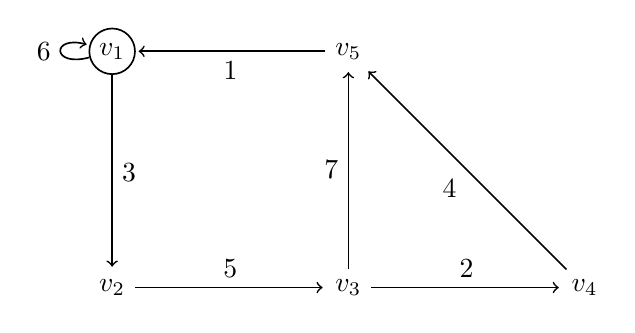
\begin{tikzpicture}[->,shorten >=1pt,auto,node distance=3cm,semithick]

    
      \node[circle, draw, fill=white, inner sep=2pt] (v1) {$v_1$};
      \node (v2) [below of=v1] {$v_2$};
      \node (v3) [right of=v2] {$v_3$};
      \node (v5) [right of=v1] {$v_5$};
      \node (v4) [right of=v5, below of=v5] {$v_4$};
    
      \path (v1) edge node {3} (v2)
            (v2) edge node {5} (v3)
            (v3) edge node {2} (v4)
            (v4) edge node {4} (v5)
            (v5) edge node {1} (v1)
            (v1) edge [loop left] node {6} (v1)
            (v3) edge node {7} (v5);
    \end{tikzpicture}
    \caption{Weighted Directed Graph with 5 Nodes}
\end{figure}

\begin{align*}
    A = \begin{bmatrix}
    \infty & 3 & \infty & \infty & \infty \\
    \infty & \infty & 5 & \infty & \infty \\
    \infty & \infty & \infty & 2 & 7 \\
    \infty & \infty & \infty & \infty & 4 \\
    1 & \infty & \infty & \infty & \infty \\
    \end{bmatrix}
\end{align*}
\section{The semiring}
\section{Einsums}
\subsection{Definition}
\subsection{Common examples}
\subsection{Properties}